
%(BEGIN_QUESTION)
% Copyright 2011, Tony R. Kuphaldt, released under the Creative Commons Attribution License (v 1.0)
% This means you may do almost anything with this work of mine, so long as you give me proper credit

This electrically-heated oven has a problem: instead of cycling between 340 $^{o}$F and 350 $^{o}$F as it is designed to, the temperature cycles between 349 $^{o}$F and 351 $^{o}$F:

$$\includegraphics[width=15.5cm]{i00296x01.eps}$$

Identify the likelihood of each specified fault for this circuit.  Consider each fault one at a time (i.e. no coincidental faults), determining whether or not each fault could independently account for {\it all} measurements and symptoms in this circuit.

% No blank lines allowed between lines of an \halign structure!
% I use comments (%) instead, so that TeX doesn't choke.

$$\vbox{\offinterlineskip
\halign{\strut
\vrule \quad\hfil # \ \hfil & 
\vrule \quad\hfil # \ \hfil & 
\vrule \quad\hfil # \ \hfil \vrule \cr
\noalign{\hrule}
%
% First row
{\bf Fault} & {\bf Possible} & {\bf Impossible} \cr
%
\noalign{\hrule}
%
% Another row
TSL contact failed open &  &  \cr
%
\noalign{\hrule}
%
% Another row
TSL contact failed shorted &  &  \cr
%
\noalign{\hrule}
%
% Another row
TSH contact failed open &  &  \cr
%
\noalign{\hrule}
%
% Another row
TSH contact failed shorted &  &  \cr
%
\noalign{\hrule}
%
% Another row
TC-1 contact failed open &  &  \cr
%
\noalign{\hrule}
%
% Another row
TC-1 contact failed shorted &  &  \cr
%
\noalign{\hrule}
%
% Another row
TC-2 contact failed open &  &  \cr
%
\noalign{\hrule}
%
% Another row
TC-2 contact failed shorted &  &  \cr
%
\noalign{\hrule}
%
% Another row
TC relay coil failed open &  &  \cr
%
\noalign{\hrule}
%
% Another row
TC relay coil failed shorted &  &  \cr
%
\noalign{\hrule}
%
% Another row
Broken wire between points C and F &  &  \cr
%
\noalign{\hrule}
%
% Another row
Broken wire between points A and B &  &  \cr
%
\noalign{\hrule}
} % End of \halign 
}$$ % End of \vbox

Finally, identify the {\it next} diagnostic test or measurement you would make on this system.  Explain how the result(s) of this next test or measurement help further identify the location and/or nature of the fault.

\underbar{file i00296}
%(END_QUESTION)





%(BEGIN_ANSWER)

% No blank lines allowed between lines of an \halign structure!
% I use comments (%) instead, so that TeX doesn't choke.

$$\vbox{\offinterlineskip
\halign{\strut
\vrule \quad\hfil # \ \hfil & 
\vrule \quad\hfil # \ \hfil & 
\vrule \quad\hfil # \ \hfil \vrule \cr
\noalign{\hrule}
%
% First row
{\bf Fault} & {\bf Possible} & {\bf Impossible} \cr
%
\noalign{\hrule}
%
% Another row
TSL contact failed open &  & $\surd$ \cr
%
\noalign{\hrule}
%
% Another row
TSL contact failed shorted & $\surd$ &  \cr
%
\noalign{\hrule}
%
% Another row
TSH contact failed open &  & $\surd$ \cr
%
\noalign{\hrule}
%
% Another row
TSH contact failed shorted &  & $\surd$ \cr
%
\noalign{\hrule}
%
% Another row
TC-1 contact failed open &  & $\surd$ \cr
%
\noalign{\hrule}
%
% Another row
TC-1 contact failed shorted & $\surd$ &  \cr
%
\noalign{\hrule}
%
% Another row
TC-2 contact failed open &  & $\surd$ \cr
%
\noalign{\hrule}
%
% Another row
TC-2 contact failed shorted &  & $\surd$ \cr
%
\noalign{\hrule}
%
% Another row
TC relay coil failed open &  & $\surd$ \cr
%
\noalign{\hrule}
%
% Another row
TC relay coil failed shorted &  & $\surd$ \cr
%
\noalign{\hrule}
%
% Another row
Broken wire between points C and F &  & $\surd$ \cr
%
\noalign{\hrule}
%
% Another row
Broken wire between points A and B &  & $\surd$ \cr
%
\noalign{\hrule}
} % End of \halign 
}$$ % End of \vbox

A good test would be to disconnect the wire between points {\bf C} and {\bf F} to see if the cycling changes at all.

%(END_ANSWER)





%(BEGIN_NOTES)

\vskip 20pt \vbox{\hrule \hbox{\strut \vrule{} {\bf Virtual Troubleshooting} \vrule} \hrule}

This question is a good candidate for a ``Virtual Troubleshooting'' exercise.  Presenting the diagram to students, you first imagine in your own mind a particular fault in the system.  Then, you present one or more symptoms of that fault (something noticeable by an operator or other user of the system).  Students then propose various diagnostic tests to perform on this system to identify the nature and location of the fault, as though they were technicians trying to troubleshoot the problem.  Your job is to tell them what the result(s) would be for each of the proposed diagnostic tests, documenting those results where all the students can see.

During and after the exercise, it is good to ask students follow-up questions such as:

\begin{itemize}
\item{} What does the result of the last diagnostic test tell you about the fault?
\item{} Suppose the results of the last diagnostic test were different.  What then would that result tell you about the fault?
\item{} Is the last diagnostic test the best one we could do?
\item{} What would be the ideal order of tests, to diagnose the problem in as few steps as possible?
\end{itemize}


%INDEX% Control, basics: differential gap control (electromechanical relay)
%INDEX% Control, basics: on/off control (with deadband)
%INDEX% Process: cookie baking oven
%INDEX% Troubleshooting review: electric circuits

%(END_NOTES)


